\section{Modeling and Simulation}
\label{sec:modeling}
For the purpose of doing design verification and optimization, a simplified model of the robot was created. The model was created in Simscape, a physical modeling toolbox integrated with MATLAB/Simulink. 
\subsection{Simscape}

Simscape is a simulation tool that allows you to rapidly create models of physical systems within Mathworks' MATLAB/Simulink environment. With Simscape, physical systems are built by interconnecting blocks representing physical components, such as rigid bodies, joints and springs in a block diagram. The blocks are parameterized by physical properties, such as mass, inertia, and damping. Simscape automatically generates the equations of motion for the system, which can be solved numerically to simulate the system's behavior. Like you can do with Simulink without Simscape, you can also add ordinary Simulink blocks, including Matlab Function blocks, to the model. Simscape is also compatible with Simulink's multiple numerical solvers, such as ode15s, ode45, and ode23s (TODO? Is it ode23t?). 

An example of a Simscape typical SimScape block diagram can be found in figure \ref{fig:simscape_tutorial_diagram}. A visualization of the corresponding model can be seen in figure \ref{fig:simscape_tutorial_visualization}, as one can see, each element in a block diagram can typically consist of a physical block, or joint blocks that lie between the physical bodies they are supposed to connect. Since a given body has multiple possible locations that a joint could be connected to, as well as axes it can act on, blocks can export different frames, with different origins and orientations, depending on the desired position and orientation of the joint. For example, for a block representing the robotic equivalent of a thigh, natural output frames would be the ones with origins at the top and bottom of the thigh, with a select axis aligned with the desired knee or hip axis of rotation. TODO: We want to use something other than the tutorial here, but our robot model is too split into submodels of submodels, so it loses the intuition you get from a "flatter" model. Will fix later. 

\begin{figure}
    \centering
    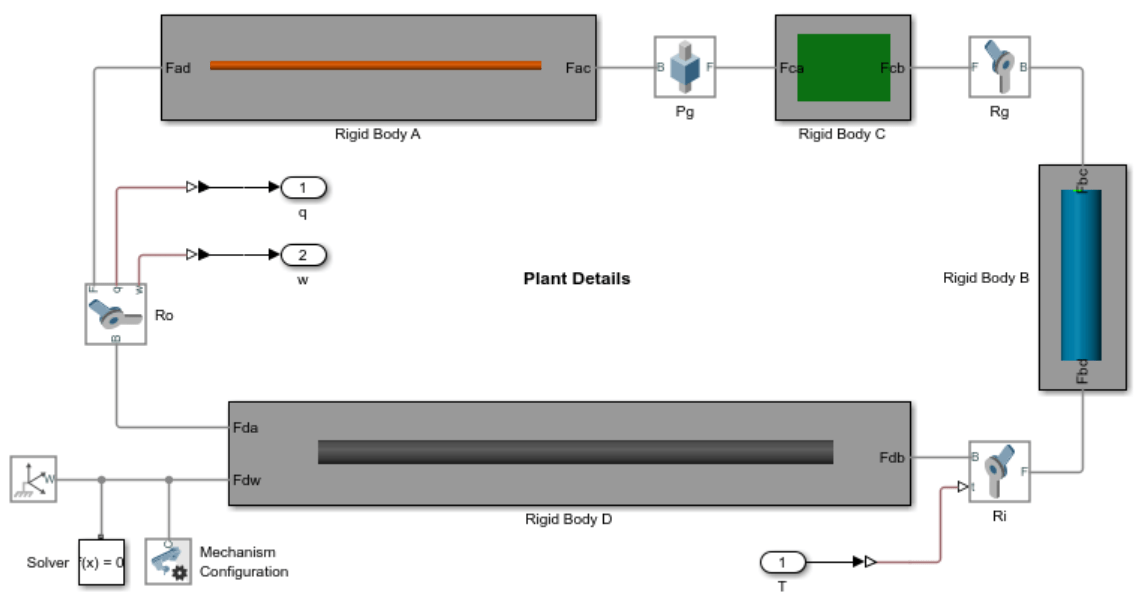
\includegraphics[width=0.5\textwidth]{Images/simscape_tutorial_diagram.png}
    \caption{A typical Simscape block diagram.}
    \label{fig:simscape_tutorial_diagram}
\end{figure}
\begin{figure}
    \centering
    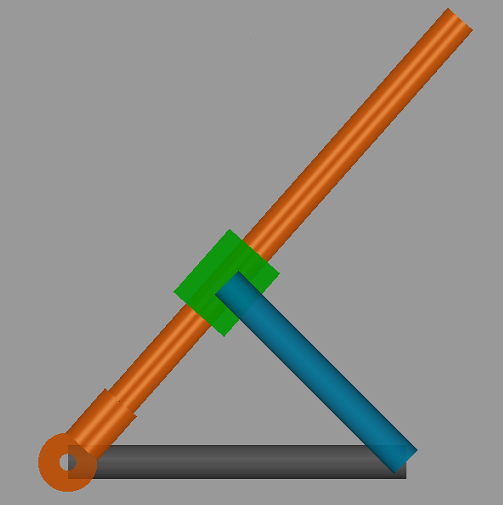
\includegraphics[width=0.5\textwidth]{Images/simscape_tutorial_visualization.png}
    \caption{A visualization of the model in figure \ref{fig:simscape_tutorial_diagram}.}
    \label{fig:simscape_tutorial_visualization}
\end{figure}

\subsection{Robot Body, Legs and Joints}
\label{sec:robot_main_parts}

Since the purpose of the Simscape model is not to develop a complicated full degree of freedom feedback controller, nor to optimize every small detail of the design, a simplified model was selected. This model consists of a main body with four legs, each of which with two degrees of freedom. A visualization of the model, as well as an overview of the body's naming conventions can be found in figure \ref{fig:name_conventions}. An overview of the body's angle conventions can be found in figure \ref{fig:angle_conventions}. Note the absence of a hip abduction/adduction joint. This is because the model's main purpose is to verify the design for jumping in the sagittal (forward-backward and upwards-downwards) plane, and the hip abduction/adduction joint is not necessary for this purpose.

Regarding the naming conventions presented in figure \ref{fig:name_conventions}, note especially the naming of the different legs corresponding to location on the body, namely RH (Right Hind), RF (Right Front), LH (Left Hind), and LF (Left Front). Note also the naming of the joints hip (HIP) and knee (KNEE). If you see the angle conventions in figure \ref{fig:angle_conventions}, you can see that the angles of these joints correspond to the angles $\theta_1$ and $\theta_2$ respectively. Note that an orientation of zero degrees for the hip joint corresponds to the leg pointing straight downwards, and an orientation of zero degrees for the knee joint corresponds to the shank pointing in the same direction as the thigh. 

TODO: Add body coordsys in both figures? So I can explain that positive rotation for both sides corresponds to positive rotation about the body y axis in nominal position. 

TODO: We also need to mention the motors, as well as what they weigh, what the legs weigh, that the legs are aluminum, how we got the main body mass, etc. 

\begin{figure}
    \centering
    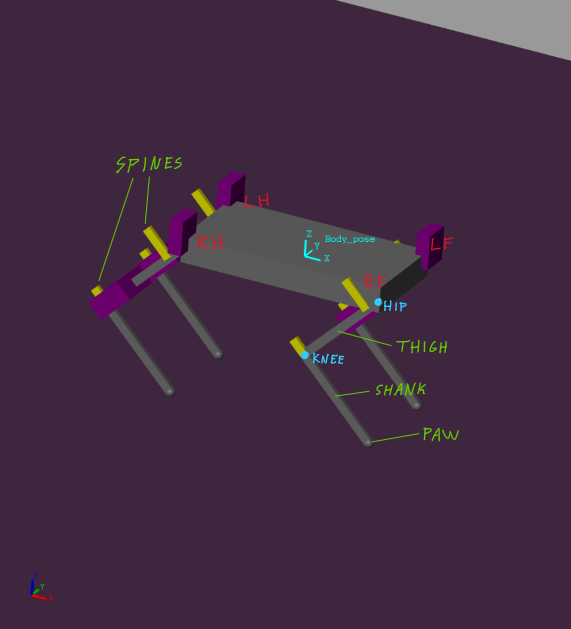
\includegraphics[width=0.5\textwidth]{Images/name_conventions.png}
    \caption{Naming conventions for the parts of the robot, as well as forwards direction definition. TODO: name spines}
    \label{fig:name_conventions}
\end{figure}

\begin{figure}
    \centering
    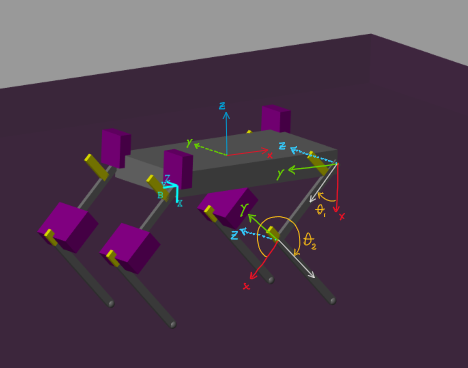
\includegraphics[width=0.5\textwidth]{Images/angle_conventions.png}
    \caption{Angle conventions for the robot body.}
    \label{fig:angle_conventions}
\end{figure}

\subsection{Elastic Components: Springs}

In addition to the model's many rigid bodies, we also implemented two different forms of spring based passive actuation, namely: 
\begin{itemize}
\item \textbf{A torsional spring} acting in parallel with the knee joint, as illustrated in figure TODO. This spring is at zero extension when the knee joint is at zero degrees, and applies a torque that is proportional to the knee joint angle, as covered in section TODO. TODO: add theory
\item \textbf{An extension spring} acting in parallel with the knee joint, attached to the shank and thigh spine, as illustrated in TODO: add figure illustrating spines/add spine description in main body figure. 
\end{itemize}

Thes were both modeled according to standard simscape way, have a simscape block diagram screenshot here, TODO. 

\subsection{Solver selection}

Mention that ode23s, and that ode15s created energy, ie. it was unphysical.

%\subsection{Simscape}
%Simscape is a physical modeling toolbox integrated with MATLAB/Simulink. While Simulink handles signal-based modeling through block diagrams, Simscape adds the ability to model physical components and their interactions directly. For this project, its multibody library was used to create a simplified model of the robot. The key advantage is automatic handling of complex multi-body dynamics equations. Rather than manual derivation, Simscape generates them based on specified geometry and joints. The model parameters can be easily modified through MATLAB scripts.

%\subsection{Motor Torque-Speed Characteristics}
%To model the motor torque-speed characteristics, a torque-speed curve such as the one covered in section \ref{sec:theory:motor_model} was used, with parameters as covered in section \ref{sec:hardware:motor_characteristics}.



%\subsection{Motor Friction Modelling}
%Since the motors will be turned off during the jumping maneuver, motor friction must be included. It was modelled using a linear motor friction model covered in section \ref{sec:theory:motor_model}, using only the viscous friction component. To estimate the model parameters, we performed hardware tests for each motor, where the motors acted as the axis of rotation for a pendulum. A aluminium rod with a aluminium ballast was attacted to the motor shaft, and the pendulum was released from rest at horizontal position and allowed to swing freely untill at rest. This was repeated for both motors. The tests where filmed by a phone camera placed at a distance in front of the pendulum, and the angles of the pendulum were manually annotated using Tracker \cite{tracker}. The hardware setup is shown in figure \ref{fig:motor_friction_test_setup}, and the results are shown in figure \ref{fig:results:motor_friction_test}.

